\documentclass[a4paper, 10pt]{report}
\usepackage{tikz}
\usetikzlibrary{angles,quotes}
\begin{document}
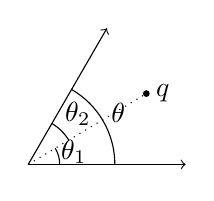
\begin{tikzpicture}
\coordinate (O) at (0,0);
\coordinate (A) at (2,0);
\coordinate (B) at (1.5,0.9);
\coordinate (C) at (1,1.73);

\draw[->](O) -- (A);
\draw[dotted](O) -- (B) node[right] {$q$};
\draw[->](O) -- (C);

\draw[fill=black] (B) circle (1 pt);

\pic [draw, -, "$\theta_1$", angle eccentricity=1.5, angle radius=4mm] {angle = A--O--B};
\pic [draw, -, "$\theta_2$", angle eccentricity=1.5, angle radius=6mm] {angle = B--O--C};
\pic [draw, -, "$\theta$", angle eccentricity=1.2, angle radius=11mm] {angle = A--O--C};

\end{tikzpicture}
\end{document}